%
% 公立はこだて未来大学卒業研究中間報告書[全コース対応版]
%
%         ファイル名:"sample.tex"
%
\documentclass[11pt]{ujarticle}
\usepackage{funinfosys}
\usepackage{url}
\usepackage[dvipdfmx]{graphicx}

\author{% 
b1020036 中川匠海\\指導教員 : 松原克弥
}
\course{Information Systems Course}

\title{キャンパスDX に向けた学務情報のオープンデータ化}
\etitle{Open Data Initiatives for Academic Affairs Information in Preparation for Campus Digital Transformation (DX)}
\eauthor{Takumi Nakagawa}
\abstract{今日の大学ではLearning Management System(LMS)や教務システムなど、目的に応じて複数のシステムを組み合わせたICT学習支援環境を構築している.しかし、複数のシステムに情報が分散していることや、Webサイトやメール等の限られたアクセス手段しか提供されないことで、学生に対する「学務情報への到達容易性」が課題となっている.
\\ 本研究では、未来大にて使用されている複数のシステムで、それぞれ異なる形式で分散管理されている学務情報(休講、補講、教室変更、振替連絡、課題〆切、教室空き情報など)をスクレイピング技術等を用いて収集し、モバイルアプリなどで活用できるようオープンデータ化し、スマートフォンやSNSなどの情報アクセス媒体になれた「デジタルネイティブ世代」の学生に適した学習支援の実現を目指す.}
\keywords{キャンパスDX,オープンデータ,公立はこだて未来大学}
\eabstract{Modern universities employ Learning Management Systems (LMS) and other systems to create comprehensive ICT learning environments. Nonetheless, the dispersion of information across various systems and limited accessibility impede students' easy retrieval of academic information.
\\In this research, conducted at Mirai University, we seek to collect disparate academic data (including class cancellations, supplementary lessons, room changes, notifications, assignment deadlines, and room availability) through scraping technology. By converting this information into open data, we aim to enhance learning support for 'digital native' students accustomed to smartphones and social networks.}
\ekeywords{CampusDX, OpenData, FUN}
\begin{document}
\maketitle
%\vspace*{-.5cm}

\section{背景と目的}

現代の教育界は、テクノロジーの急速な進展に伴い、その運営方法と学習環境に著しい変化を見せている。特に、キャンパスのデジタルトランスフォーメーション(以降キャンパスDXと表記)が全国的な規模で急速に加速しており、リモート授業、デジタル教材の使用、オンライン評価システム、データ分析など、教育のデジタル化は急速に進行している。

この動向は他大学でも顕著である.例えば、立教大学では、授業スケジュールに応じた教室の空き状況をリアルタイムで把握できる「立教大学シラバス検索システム」が実装されている.このシステムでは、特定の曜日と時限にどの教室が空いているのかが一目でわかるため、学生は授業や自習の計画を用意に建てることができる[1].また、東京学芸大学では、非公式の「東京学芸大学今日右室検索システム」が存在し、こちらも授業で使用されている教室と秋教室が一覧で表示される.このシステムは、自習などの目的で利用する場合、特に推奨される教室を強調表示する機能も備えている[2].

この結果として、学務情報へのアクセス性や柔軟性が大幅に向上しているが、新たな課題も浮上している.

未来大では、教育プロセスの多くがデジタル化されている一方、重要な学務情報が複数のWebサイトに分散しており、学生が情報へのアクセスの困難さが問題となっている。具体的に、学生が必要とする情報は、教務システム(Student)、LMS(HOPE)、情報ライブラリサイト、未来大公式ホームページなど、異なるプラットフォームに散在している。これにより、学生は必要な情報を効率的に検索し、アクセスすることが困難になっており、学習経験に影響を与える可能性があります。

さらに、現行のシステムは情報更新時に学生へ能動的な通知機能が欠如している.この状況では、学生は自らWebサイトへ主体的に情報を取得する必要のある"pull型"アプローチとなっている.従って、情報が更新された際に、その内容を自動的に学生に伝える"push型"の通知型メカニズムが存在しない現在は、学生が重要な情報の更新を見逃す危険性を増大させる要因となっている.これにより、学生の情報アクセスの効率が低下し、学習における不都合を招く可能性が高い.こうしたことから、学務情報への情報到達容易性を向上させることの重要性が高まる.

%目的

そこで本研究の目的は、スクレイピング技術を活用して、未来大の学務情報をオープンデータ化することによる情報到達容易性向上を目的とする.学務情報のオープンデータ化により、分散している情報源からのデータ収集と統合が可能となり、学生にとって重要な情報への迅速かつ一元的なアクセスを実現する.

デジタル化された教育環境においては、情報のアクセシビリティが学生の学習成果に直結している.本研究を通じて、未来大のキャンパスDXを一層推進し、デジタルネイティブ世代の学生にとって、より効率的かつ効果的な学習環境を提供することが期待される.


\section{スクレイピング}

スクレイピングは、Webページから情報を自動で取得・抽出する技術である.

具体的には、WebページのHTMLやXMLデータを解析し、必要な情報をプログラム的に取り出すプロセスを指す.この技術は、多岐にわたる分野で用いられ、特にデータ解析や機械学習の領域でデータ収集手段として注目を浴びている.

スクレイピングな基本的な手法として、まずHTTPリクエストを使用して目的のWebページのデータを取得します.このプロセスは、Webクローラーというプログラムを用いて、自動的に複数のWebページを巡回し、データを収集することが一般的である.得られたデータから特定の情報を抽出するために、DOMパーサーや正規表現などの方法を使用する.これにより、大量のWebページから一貫した形式でデータを収集することが可能となる.

\begin{figure}[h]
	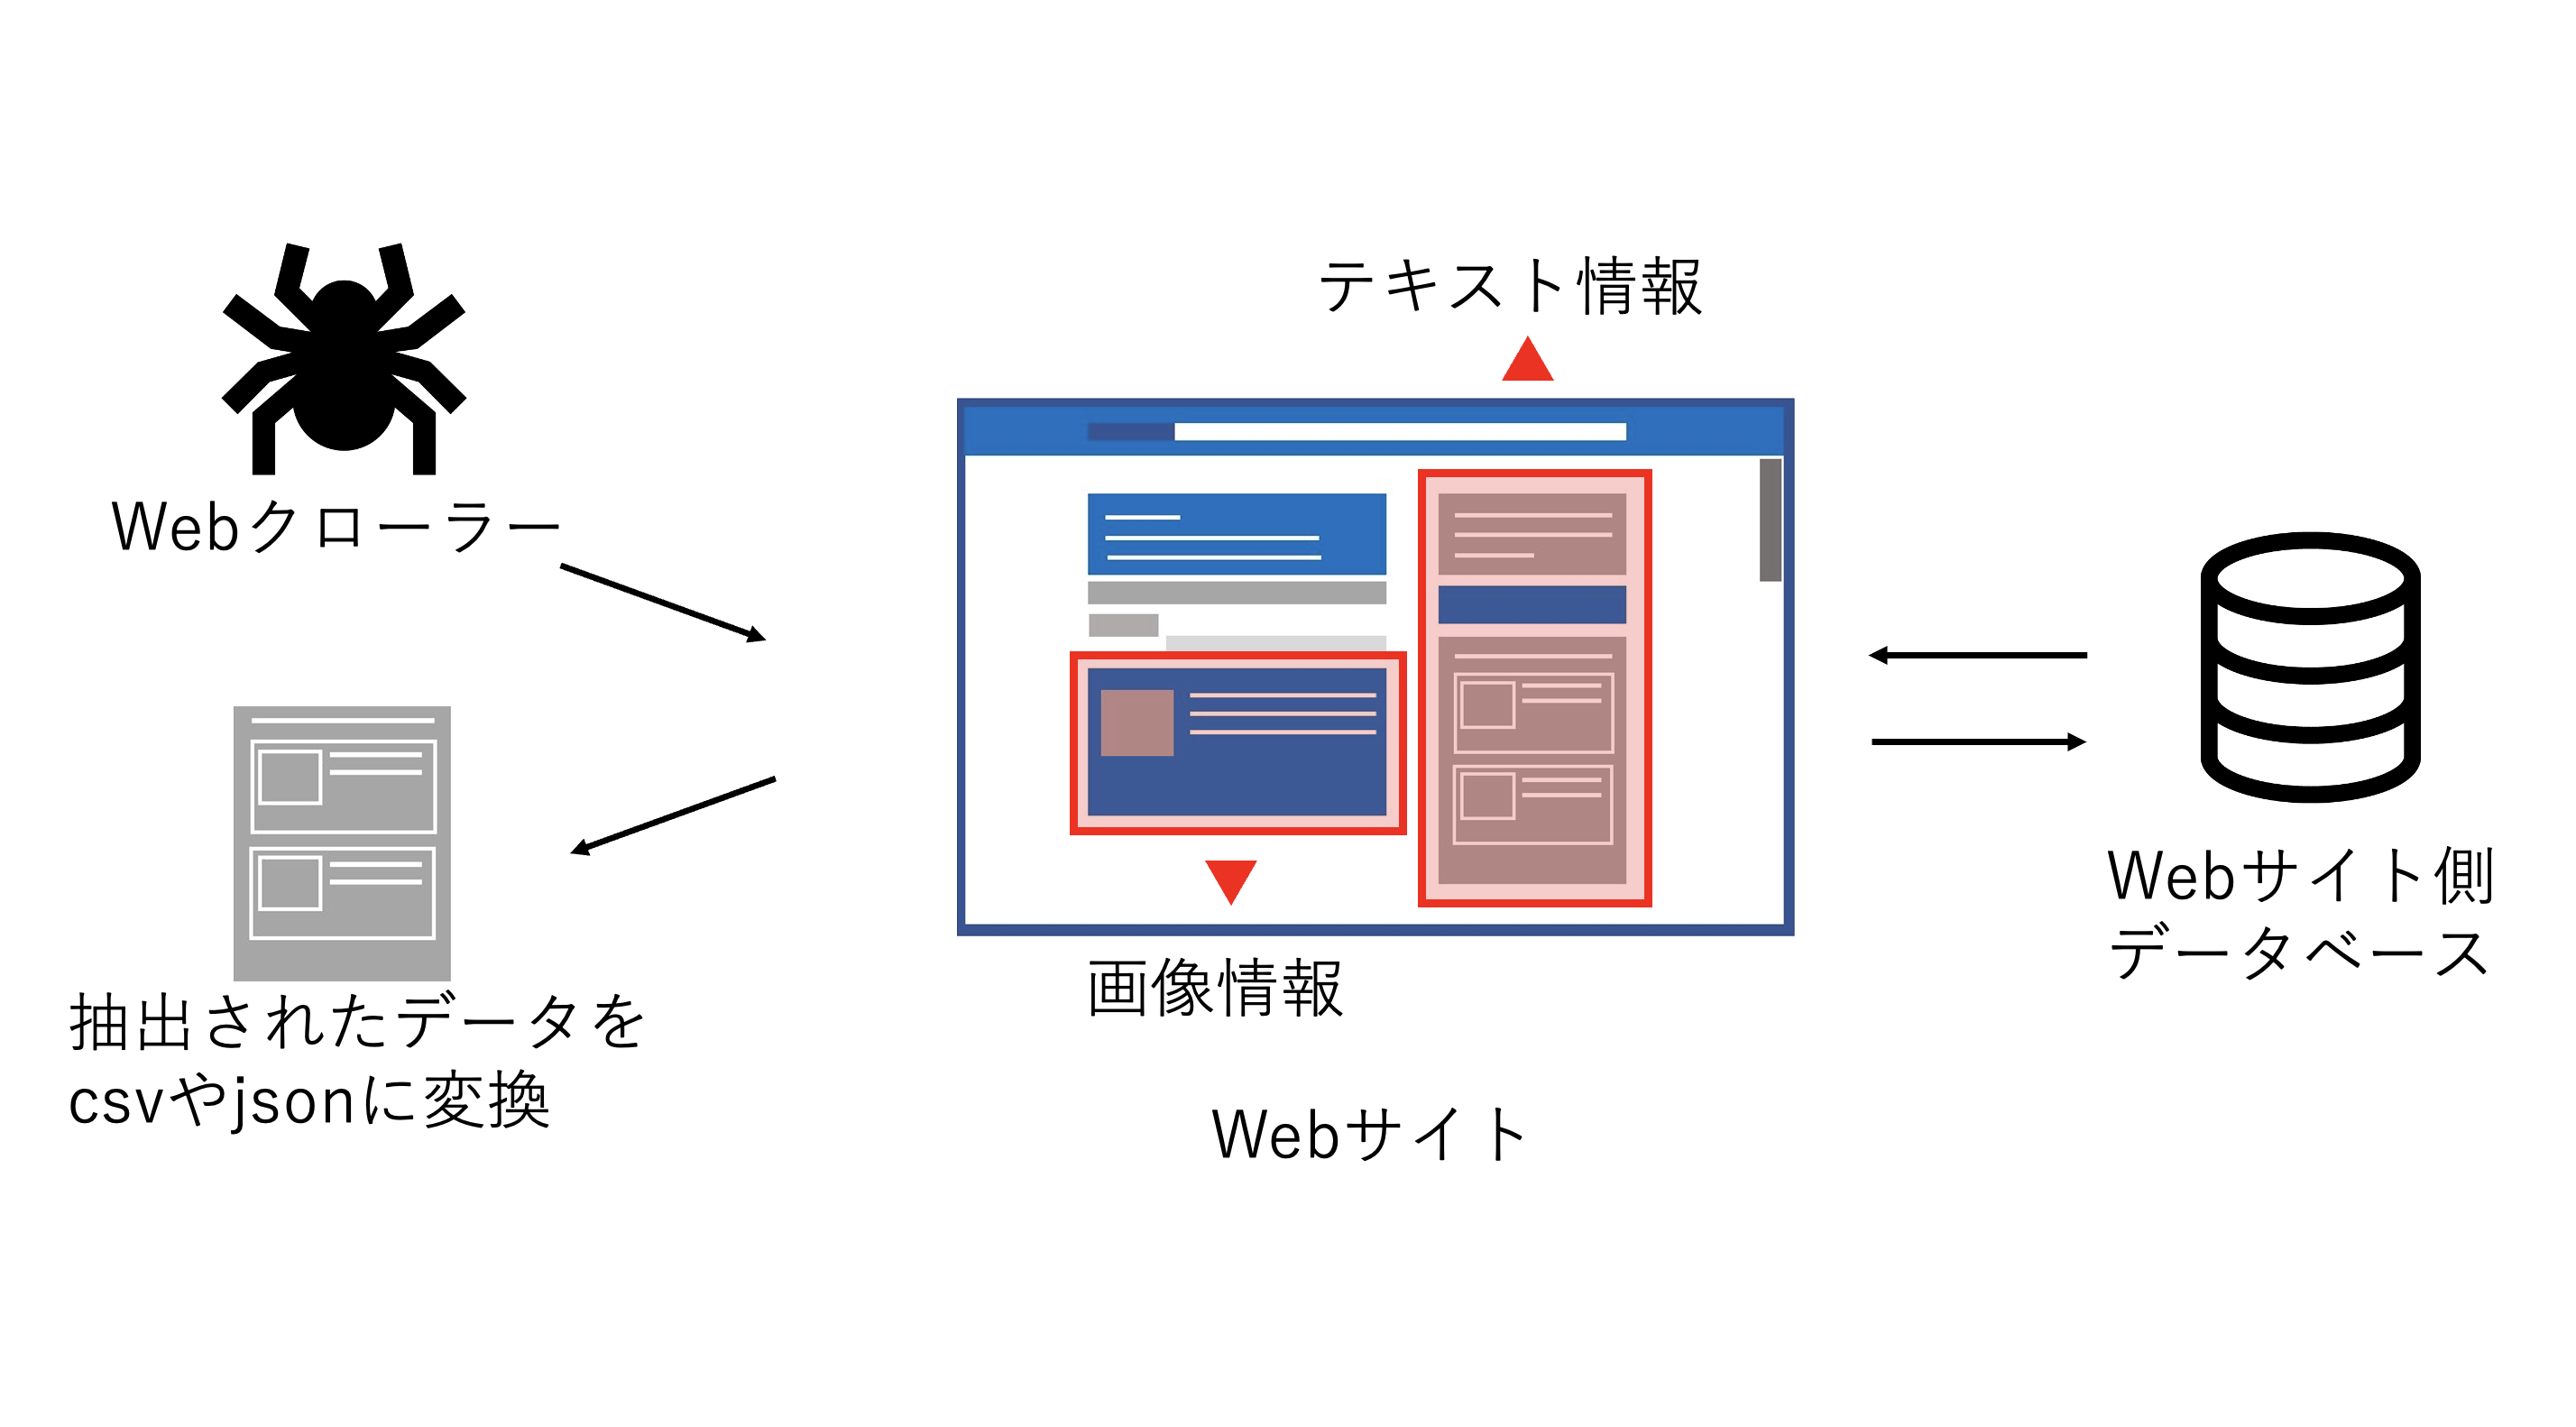
\includegraphics[width=0.9\linewidth]{./src/selenium.png}
	\caption{スクレイピングの解説}
  \label{fig:arch}
\end{figure}

\section{提案}

本研究では、スクレイピングを用いて未来大の学務情報をオープンデータとして提供し、情報到達容易性を向上させることである.

前述の通り、未来大の学務情報は現状複数のWebサイトに分散しているため、情報アクセスの効率が低下している.学務情報をオープンデータとして公開することによって、モバイルアプリなど他システムで活用できるようになり、情報の分散問題の解消や、情報アクセスの障害が低減することが期待される.
また、本提案のプラットフォームには、新たに”push型"の通知型メカニズムを導入する.これによって、現状学生が自主的に学務情報を取得しに行かなくてはいけない"pull型"から変更され、学生が自動的に通知を受け取る事ができ、情報の取得が効率的となる.この機能は学生が最新の情報にアクセスできるようにするための重要な要素である.


\section{実装}

本研究において、既存のWebサイトから学務情報を自動的に取得するためのスクレイピングツールとしてSeleniumを採用する.Seleniumは、動的なWebページやログインが必要なページの自動操作を得意とするブラウザ操作ツールである[3].このツールは、未来大の教務システムのような動的に内容の変わるWebページや、認証が要求されるページに置いて特に効果を発揮する.

システムの具体的な動作として、クライアントの要求を受け、Seleniumを使用して教務システムにログインし、学務関連の情報を取得する.対象とする情報は、大学からのお知らせ、学生個人の成績、時間割、休講、補講、教室変更、そして施設予約状況といった主要な項目を含む.取得したデータは、json形式に変換し、クライアントへレスポンスとして返送する.
さらに、取得した情報の利用を最大化するため、該当情報を中心としたモバイルアプリケーションの実装も行う.このアプリケーションにより、情報の一元化や、更新情報のpush型通知を行えるようにする.



また、本システムに置いてセキュリティの面で、取得した学務情報や学生の認証情報の安全性が最重要視される.そのため、サーバ側でこれらの情報を保存することは避けられており、代わりに情報は一時的なメモリ上でのみ取り扱われる方式を採用する.この情報はレスポンスが生成された直後に破棄される.特に、学生がシステムを利用する際のIDとパスワードといった認証情報の取り扱いは、さらなる注意を払う必要がある.IDパスワードを送受信する際には暗号化を行い、学生の個人情報が漏洩しない設計を行う.さらに、スクレイピングによって取得したデータ、学生個人の認証情報は、サーバにデータが残存し続けると、学外へ公開できない情報の漏洩や、他学生の情報の取得が可能になってしまわないよう、メモリに一時保存し送信し終えたものは必ず破棄するシステムを実装する.

\section{進捗と計画}

進捗状況として、Seleniumを用いて教務システムのスクレイピングを行い、クライアントへのレスポンス機能を実装した.現在はよりユーザビリティの高いサービス実現のため、スクレイピングによって取得したデータの破棄機能や、IDパスワードの完全破棄、機密性の向上、レスポンスの処理速度向上に取り組んでいる.

その後の計画として、ユーザビリティ向上の実装が終わった後に実稼働への移行を行う.実稼働への以降に際し、システムのスケーラビリティとロードバランシングの効率化を重要な焦点としてアップデートを行っていく.Apacheサーバを使用し、クラウドベースのリソース活用の最適化を目指す.

実装後はモバイルデバイスでの未来大生向けモバイルアプリの実装を行う.本システムを利用し、実際に未来大での空き教室情報の閲覧や、お知らせ等の情報を学生へ自動的に伝えるpush型通知形態での設計を行い、実際に未来大生によるユーザーフィードバックを行う.

\section{まとめ}

本研究では、未来大の学務情報のオープンデータ化によるキャンパスDXの促進を目的とする.未来大において、現状の学務情報の分散と、pull型による情報取得手段しかないという、情報の取得手段が少ない現状となっている.そのため、スクレイピング技術を利用して未来大の学務情報をオープンデータ化し、オープンデータを利用して他のモバイルアプリなどから、push型による情報の取得手段の拡張と、情報到達容易性の向上によるキャンパスDXの促進を行う.

今後の課題として、スクレイピングによって取得する情報や、学生の持つIDやパスワードの漏洩を防ぐセキュリティ面の徹底がある.セキュリティの向上を行った後に、オープンデータとして利用できそう実装を行い、本システムを用いたモバイルアプリの開発と評価実験を行う.

\section{情報システムコースにおける本研究の位置づけ}

情報システムコースでは、安心・安全・快適な情報社会を支援する観点から、価値のある情報システムの創造、効率性と信頼性を考慮した情報システムの実現、多様で大規模な情報の生成と分析に関する具体的な課題に取り組み、その結果の評価を通じて、新しい方法論や、学問領域を切り拓く能力を育むことが、カリキュラムポリシーの卒業研究に対する項目として挙げられている.

本研究では、スクレイピングにより学務情報をオープンデータ化することによって、分散した学務情報の効率化を行い、キャンパスDXの促進を目標としている.これは、未来大での生活を情報システムによって支援するものであり、新しい価値の創造と実現、そして大規模な情報の生成と分析と言える.今後、実装したシステムと、システムを活用したモバイルアプリによる評価実験を行うことで、カリキュラムポリシーの「結果の評価を通じて、新しい方法論や学問領域を切り拓く能力を育む」ことに繋がる.

\begin{thebibliography}{99}
	\bibitem{rikkyo}
	立教大学, "立教大学シラバス検索システム", 立教大学. [Online]. Available from: \url{https://www.rep-rikkyo.com/class_rooms?day=c&hour=4}. Accessed: 2023-10-25.
	\bibitem{gakugei}
	東京学芸大学 (非公式), "東京学芸大学教室検索システム", 東京学芸大学. [Online]. Available from: \url{https://u-gakugei-uoa.pages.dev/akitan/}. Accessed: 2023-10-25.
	\bibitem{selenium}
	SeleniumHQ, "Selenium Documentation", Selenium, 2023. [Online]. Available from: \url{https://www.selenium.dev/documentation/en/}. Accessed: 2023-10-25.
\end{thebibliography}
\end{document}
%
%
% EOF 
